\chapter{Statement of the Problem}
\label{sec:problem}

\section{Types of Biometrics} Biometrics has been an active field of research over the last decade. The reason behind their success is that biometric characteristics are universal, unique and permanent. Unlike other forms of authentication such as passwords or identification cards which can be stolen or faked easily.

There are many kinds of biometrics which can be used for authentication purposes. Among them the prominent being, Face, Ear, Palm, Fingerprint, Iris and others which are frequently being used these days in day to day life to authenticate an individual. Another reason biometrics have been used these days are due to terrorist activities and other fraudulent ways in which people impersonate themselves which are harder to catch. These days biometrics are used everywhere from Airports to ATMs to secured entry to corporate offices where checking the identity of an identity of an individual is mandatory before access is given. It helps to strengthen the security of an organization or country potential threat. As mentioned above, the different types of biometrics, different biometrics have different purposes and importance. The most popular being face recognition which is being used everywhere to authenticate people, the only disadvantage being the change in facial expression and with age the face changes upto a certain extent which makes it difficult to recognize and authenticate. Fingerprint is also being used in almost any high priority zone nowadays to authenticate and is very successful but it requires complete co-operation of an individual in order to authenticate them. The same problem happens with iris authentication where it becomes very difficult to extract the iris image to match and authenticate. 

Ear authentication comes to the rescue in such a situation due to many reasons. The primary being the stability in the human ear structure and ear images can easily be captured without the co-operation of an individual. Each ear is unique, so any side image of an individual is enough in order to authenticate a person.

\section{Purpose of Biometric Ear Recognition} 

Ear authentication and recognition is being considered as one of the most innovative processes as of today. The human ear can be divided into six main parts: Outer helix,
the antihelix, the lobe, the tragus, the antitragus and the concha. The shape of the outer ear evolves during the embryonic state from six growth nodules. The structure is completely random, the randomness can be observed by comparing the left and right ear of the same person - thus they are not symmetric. French criminologist Alphonse Bertillon was the first to be aware of ear to be used for human identification purposes. His work was carried on by Alfred Ianarelli whoc collected 10,000 ear images and determined 12 characteristics needed to identify a person. He also conducted studies on twins and triplets thereby discovering that ears are unique even among genetically identical persons \cite{pflug2012ear}. The different parts of the ear are shown in Figure \ref{fig:Figure2}

\begin{figure}[t]
	\DeclareGraphicsExtensions{.pdf,.png,.jpg}
	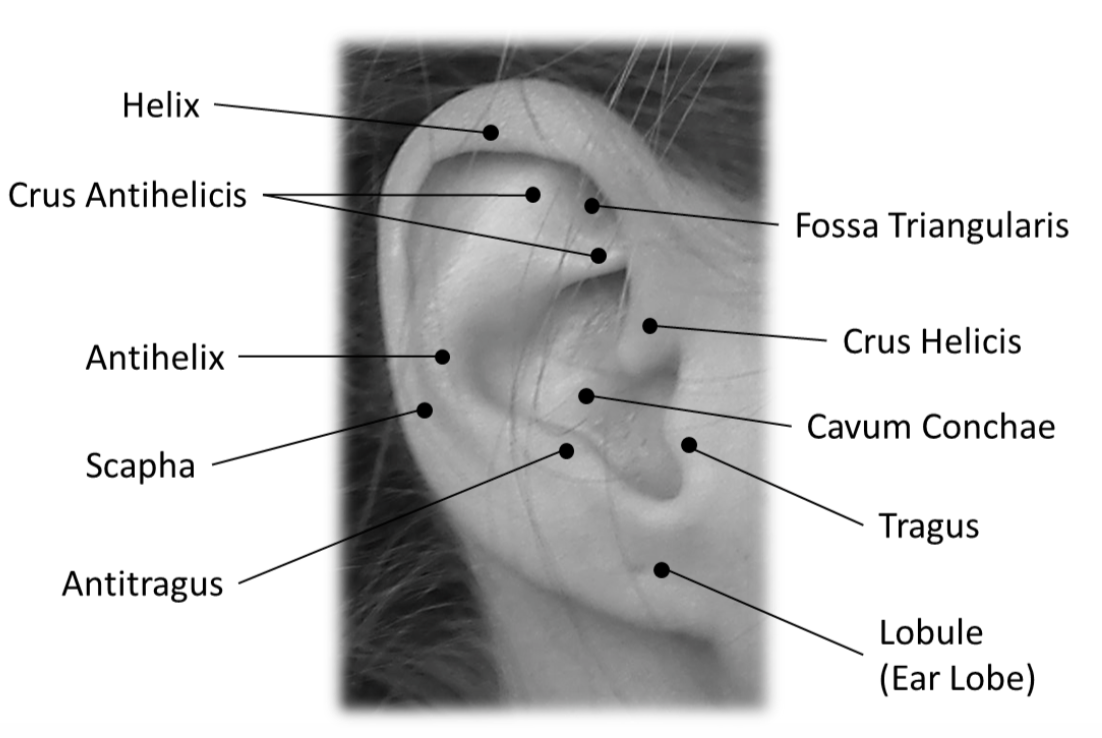
\includegraphics[width=\textwidth]{Figures/Figure2}
	\caption{Characteristics of Human Ear\cite{pflug2012ear}} 
	\label{fig:Figure2}
\end{figure}
The typical ear biometric system can be viewed as a system where an input image can be reduced to a set of features that is used to compare with the features of other images to determine its identity. The salient features of a classical ear recognition system are\cite{abaza} 

\begin{enumerate}
\item Ear Detection/ Segmentation - The first stage which is used to localize the position of the ear in the image.
\item Ear Normalization and Enhancement - The size of the ear image is normalized for standardization and enhanced using standard image processing techniques in order for more features to be extracted.
\item Feature Extraction - Feature extraction refers to a process in which the ear image is being reduced to a mathematical model called a feature vector to get information.
\item Matching Features - The features extracted are then compared to the features that are extracted earlier and stored in the database to find a match.
\item Decision - Matching scores are generated by the model used to train the features to give a decision of whether the image is matched or not.
\end{enumerate}

\section{Contributions of this Project} The main goal of this work is to develop
shallow and deep techniques to extract efficient features from a set of ear images in order to authenticate a human being. A thorough comparison of two traditional techniques called SIFT(Scale-Invariant Feature Transform)[] and SURF(Speed-up of Robust Features have been provided)[], then another comparison has been done with modern deep learning models constructed with the help of convolution neural networks[].  \cite{harris}. My paper is \cite{sarkar}
